\subsection{Momento de torsión sobre una espira}

Es importante que antes de abordar esta sección se haya entendido bien la sección anterior (\ref{sec:fuerza_magnetica_en_un_conductor}) y que recuerde qué es torque. Si desea ver un recordatorio sobre torque puede utilizar el resumen dado en la sección \ref{sec:torque_y_momento_de_inercia}.

\subsubsection{Definición de espira}

Tal vez parezca trivial definir el concepto de espira, sin embargo vamos a aclarar los elementos que vamos a usar para demostrar cómo generamos el par de torsión. Entonces, una espira es un lazo de alambre por el que puede fluir corriente eléctrica. Vamos a tomar una espira rectangular, y vamos a suponer que fluye una corriente como se muestra en la figura \ref{fig:espira_vista_superior}. En este caso estamos ignorando de dónde proviene la corriente eléctrica, y suponiendo que la espira es totalmente cerrada.
\begin{wrapfigure}{l}{0.3\textwidth}
  \centering
  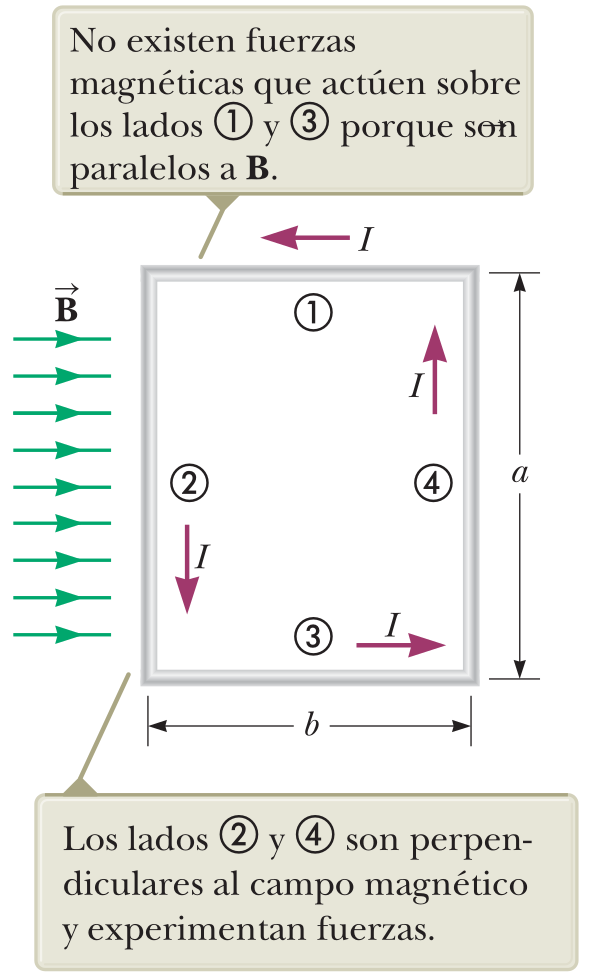
\includegraphics[width=\linewidth]{espira_sup.png}
  \caption{Vista superior de una espira rectangular}
  \label{fig:espira_vista_superior}
\end{wrapfigure}

Cuando la corriente pasa a través de la espira, las cargas fluyen a través del conductor (de la misma forma que vimos en la sección anterior). Si se coloca en un campo magnético uniforme \(\vec{B}\) de modo que sea perpendicular a dos de los segmentos (el segmento \textcircled{2} y \textcircled{4} en caso de la figura \ref{fig:espira_vista_superior}), cada uno experimenta una fuerza magnética dada por la ecuación \eqref{eq:fuerza_magnetica_en_un_conductor} mientras que en los segmentos \textcircled{1} y \textcircled{3} la fuerza magnética será nula ya que el vector \(\vec{v}_d\) y \(\vec{B}\) son paralelos. 

Las fuerzas que actúan sobre los segmentos \textcircled{2} y \textcircled{4} no se cancelan completamente en su efecto mecánico: aunque su suma vectorial puede ser nula (es decir, no producen una traslación neta de la espira), sí generan un momento de torsión o torque que tiende a rotarla.

Entonces, teniendo en cuenta que la longitud de los segmentos \textcircled{2} y \textcircled{4} es \(L=a\), el módulo de la fuerza que siente cada segmento será:
\begin{equation}
  F_{2} = F_{4} = IaB
  \label{eq:fuerza_torque_en_una_espira}
\end{equation}

\begin{tcolorbox}[myconclusion]
  Recuerda: Esta fuerza es perpendicular tanto al elemento de corriente como al campo magnético.
\end{tcolorbox}

\subsubsection{Definición de momento de torsión}

\begin{wrapfigure}{l}{0.3\textwidth}
  \centering
  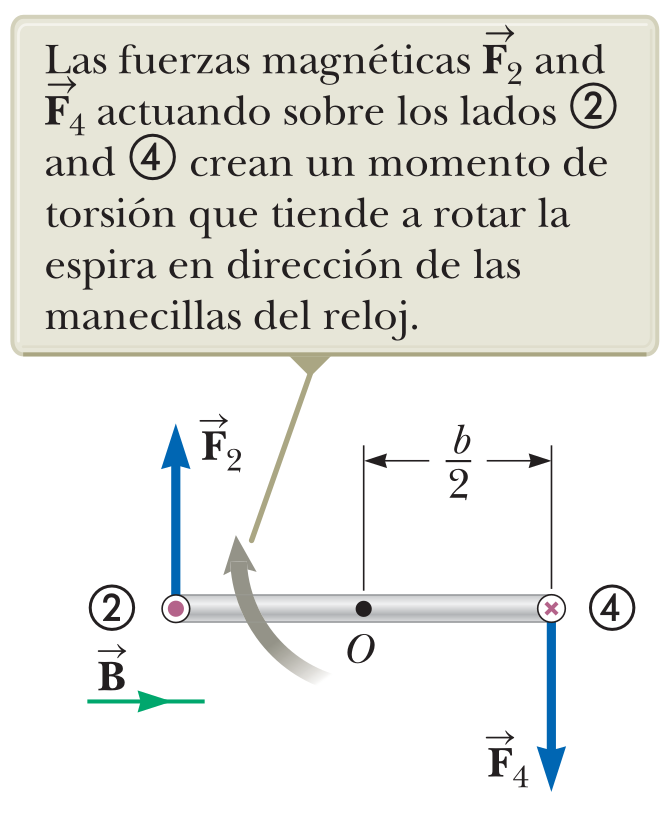
\includegraphics[width=\linewidth]{espira_lat.png}
  \caption{Vista lateral de la espira rectangular}
  \label{fig:espira_vista_lateral}
\end{wrapfigure}
Si analizamos la misma espira de la figura \ref{fig:espira_vista_superior} pero vista desde el lateral para poder visualizar las fuerzas actuantes podemos ver por qué se produce un torque.

Si se aplica la regla de la mano derecha en la figura \ref{fig:espira_vista_superior} podemos ver que en el segmento \textcircled{2} la fuerza es saliente y en el segmento \textcircled{4} la fuerza es entrante. Si vemos la figura \ref{fig:espira_vista_lateral} donde se muestra la misma espira en vista lateral, vemos que sobre el segmento \textcircled{2} la fuerza actúa hacia arriba y sobre el segmento \textcircled{4} actúa hacia abajo. Estas fuerzas no pueden provocar una traslación ya que se cancelan entre sí, pero si pueden provocar una rotación respecto de un eje \(O\).

Sabemos que el módulo del momento de torsión o torque (\(\tau\)) respecto de un eje de giro \(O\) es:
\begin{align*}
  \tau &= F\, r \sin(\theta) \\
  \text{Y}&\,\text{para dos fuerzas actuantes:}\\
  \tau &= \tau_1 + \tau_2 \\
  \tau &= F_1 r_1 \sin(\theta_1) + F_2 r_2 \sin(\theta_2)  
\end{align*}

En nuestra espira, el ángulo \(\theta=\pi/2\) será el mismo para las dos fuerzas \(F_{2}\) y \(F_{4}\), ya que depende del ángulo de la espira con \(\vec{B}\).

En base a esto, entonces observando la figura \ref{fig:espira_vista_lateral} podemos aplicar la expresión de torque a las fuerzas que actúan sobre la espira, resultando:
\begin{align}
  \tau &= F \, r \, \sin(\theta); \quad \text{donde para cada lado: } F=F_B ~~\text{y}~~ r=b/2 \nonumber \\ 
       &= F_{2} \, \frac{b}{2}\, \sin(\theta) + F_{4} \, \frac{b}{2}\, \sin(\theta) \nonumber \\
       &= \left(IaB + IaB\right)\, \frac{b}{2} \, \sin(\theta); \quad \text{donde:}~~ L=a \nonumber \\ 
       &= 2IaB \, \frac{b}{2} \, \sin(\theta) \nonumber \\
       &= IB \, ab \, \sin(\theta); \quad \text{como} ~~ A=ab \nonumber \\
  \tau &= IB \, A \, \sin(\theta)
  \label{eq:torque_para_una_espira}
\end{align}

En este caso como \(\theta = \pi/2\) se obtiene el torque máximo \(\tau_{max} = IAB\), sin embargo la expresión \eqref{eq:torque_para_una_espira} funciona para cualquier ángulo \(\theta\) que forme la espira con respecto a \(\vec{B}\). 

Sabemos que como el torque es definido como producto vectorial entonces \(\tau\) es un vector perpendicular al plano formado por otros dos vectores. En el caso de la espira, como vimos durante el desarrollo \eqref{eq:torque_para_una_espira} sabemos que el campo magnético \(\vec{B}\) es un vector. El otro vector será el área \(\vec{A}\) y, al igual que lo definimos en el flujo eléctrico y magnético, es un vector perpendicular a la superficie. Para comprender mejor el vector área de la espira, puede observarlo en la figura \ref{fig:espira_rotada}

\begin{figure}[ht]
  \centering
  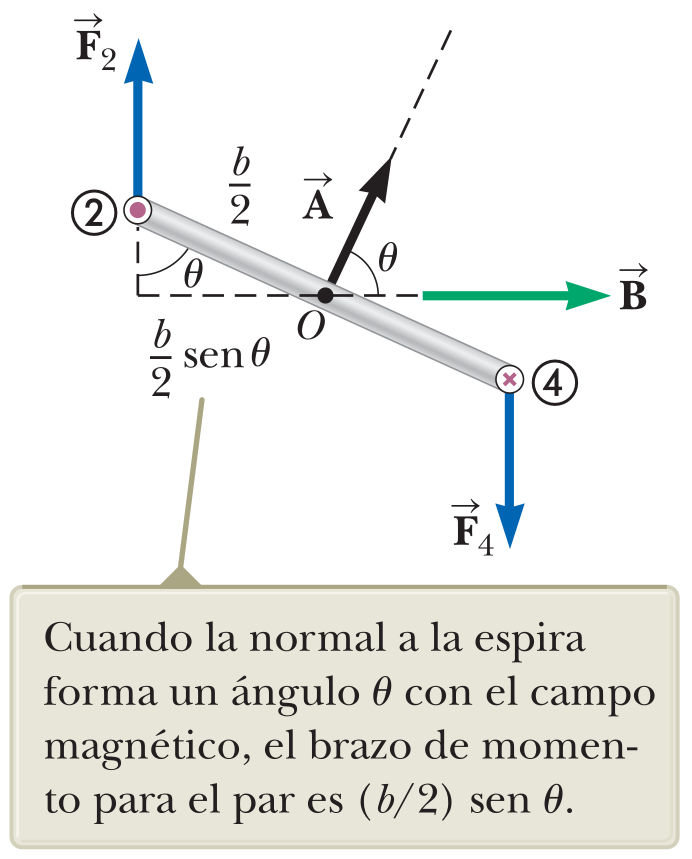
\includegraphics[width=0.4\textwidth]{espira_lat_theta.png}
  \caption{Vista lateral de la espira rectangular rotada un ángulo \(\theta\)}
  \label{fig:espira_rotada}
\end{figure}

En base a esto entonces decimos que \(\vec{tau}\) para una espira es:
\begin{equation}
  \boxed{\vec{\tau} = I\vec{A}\times \vec{B}}
  \label{eq:vec_torque_de_espira}
\end{equation}

Aunque la ecuación \ref{eq:vec_torque_de_espira} se dedujo para una espira rectangular, es válida para una espira plana de cualquier forma.

\subsubsection{Momento dipolar magnético}

El \textbf{momento dipolar magnético} de una \textit{espira} es una \hl{cantidad vectorial} que caracteriza la intensidad y la orientación del campo magnético generado por una corriente eléctrica que circula por una espira cerrada\footnote{En el Sistema Internacional, se mide en \(\text{A·m}^2\) (amperio-metro cuadrado).}.
\[
  \vec{\mu} = I \vec{A}
\]

\begin{wrapfigure}{r}{0.27\textwidth}
  \centering
  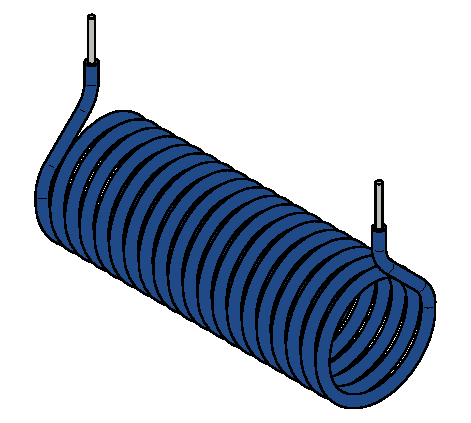
\includegraphics[width=\linewidth]{Solenoid.pdf}
  \caption{Imágen de un solenoide}
  \label{fig:solenoide}
\end{wrapfigure}
Su magnitud está dada por el producto de la corriente eléctrica (\(I\)) que fluye por la espira y el área (\(A\)) encerrada por esta:  
\[
  \mu = I A
\]  
Si se tiene un solenoide de \(N\) vueltas (o espiras), el momento se amplifica:  
\[
  \mu = N I A
\]

\begin{tcolorbox}
  \textbf{Nota}: el término \textit{espira} se suele usar para referirse a un solo lazo de alambre, mientras que un solenoide consiste en múltiples espiras enrolladas en forma de cilindro como se muestra en la figura \ref{fig:solenoide}.
\end{tcolorbox}

\(\vec{A}\) es el vector área de una sola espira o vuelta, su magnitud es el área \(A\) de la espira (por ejemplo en la figura \ref{fig:dipolar_magnet_moment} el área de la espira será \(A=\pi r^2\)), y su dirección es normal al plano de la espira, siguiendo la regla de la mano derecha respecto al sentido de la corriente. Si los dedos de la mano derecha se curvan en el sentido de la corriente, el pulgar apunta en la dirección del vector momento dipolar magnético (\(\vec{\mu}\)), perpendicular al plano de la espira.
\begin{figure}[ht]
  \centering
  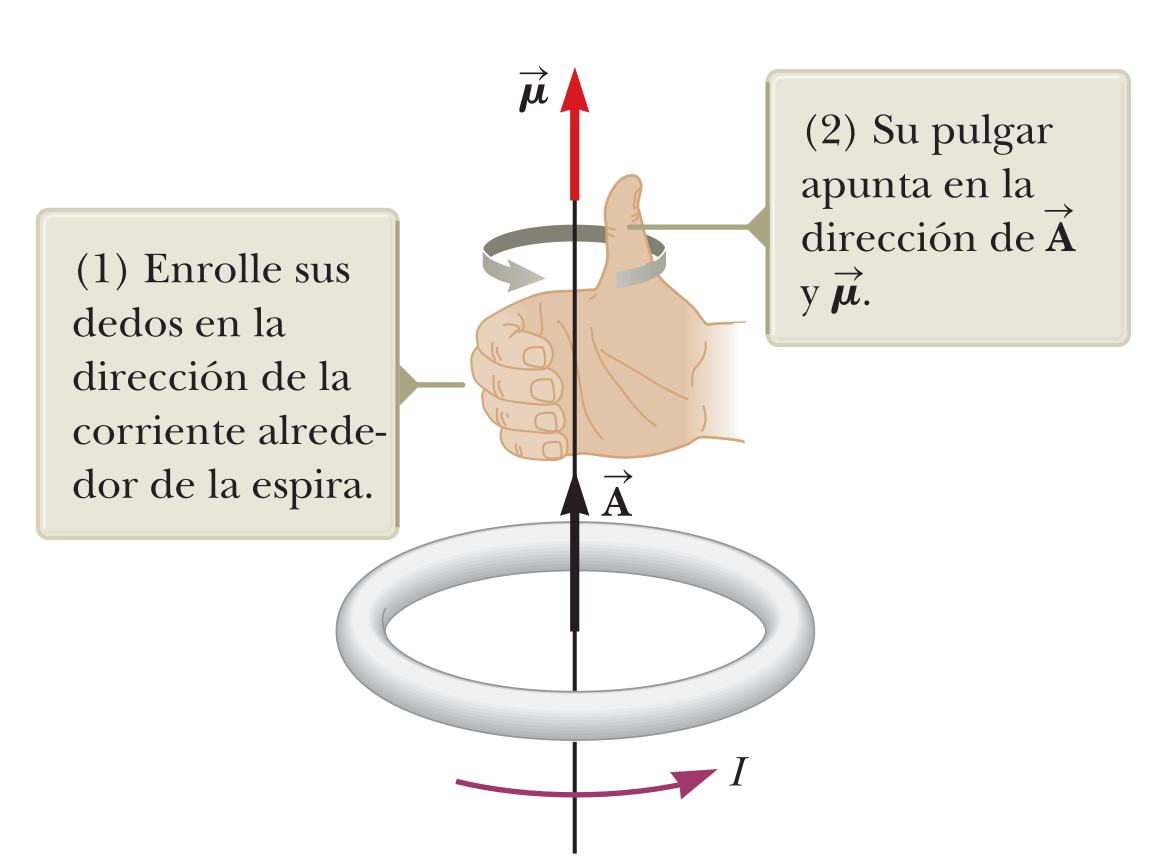
\includegraphics[width=0.5\textwidth]{dipolar_magnet_moment.png}
  \caption{Regla de la mano derecha para determinar la dirección del vector \(\vec{A}\) y el momento dipolar magnético \(\vec{\mu}\).}
  \label{fig:dipolar_magnet_moment}
\end{figure}

En base al momento dipolar magnético, se puede escribir una expresión de torque (\(\vec{\tau}\)) que experimenta un solenoide de \(N\) vueltas en presencia de un campo magnético externo (\(\vec{B}\)): 
\[
  \vec{\tau} = \vec{\mu} \times \vec{B}
\]

Si el momento magnético \(\vec{\mu}\) es paralelo al campo \(\vec{B}\), no hay momento de torsión (\(\tau = 0\)). Si \(\vec{\mu}\) es perpendicular a \(\vec{B}\), el momento de torsión es máximo. El torque tiende a alinear \(\vec{\mu}\) con \(\vec{B}\).

\begin{figure}[ht]
  \centering
  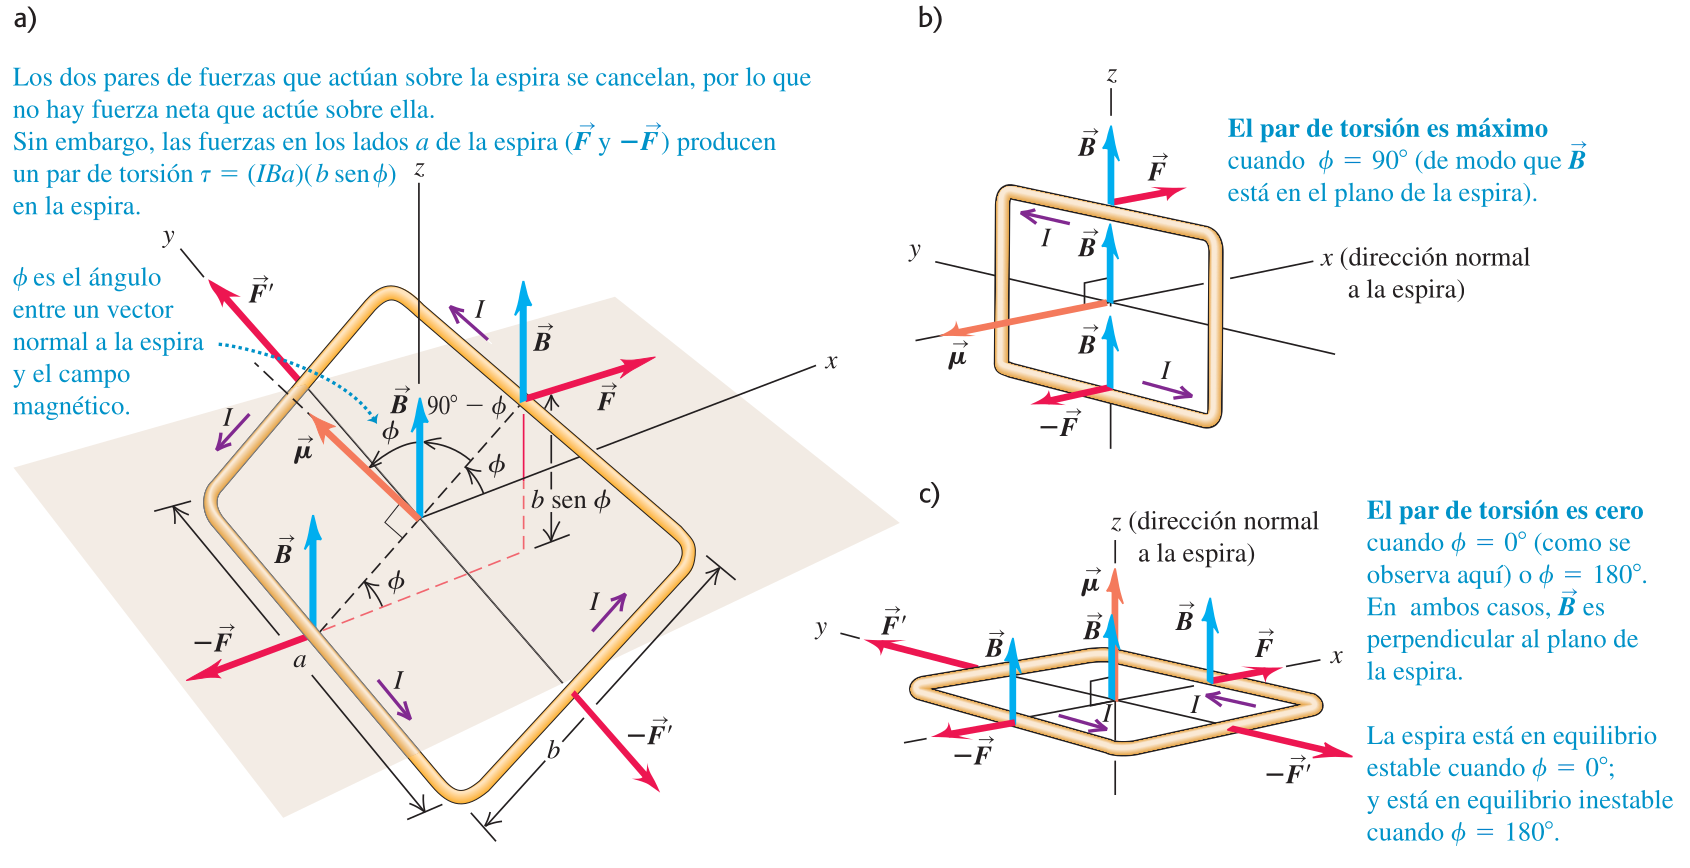
\includegraphics[width=1\textwidth]{par.png}
  \caption{Cálculo del par de torsión sobre una espira que conduce corriente en un campo magnético uniforme.}
\end{figure}

\begin{tcolorbox}[myconclusion]
  El momento magnético mide cuán magnético es un cuerpo, en el mismo sentido que el momento angular mide cuán rotacional es, y el momento lineal cuán translacional.
\end{tcolorbox}

Cuando un sistema con momento magnético \(\vec{\mu}\) se coloca en un campo magnético externo \(\vec{B}\), experimenta:
\begin{itemize}
  \item \textbf{Un torque}: \(\vec{\tau}=\vec{\mu}\times\vec{B}\) que lo alinea con el campo,
  \item \textbf{Una energía potencial}: \(U=-\vec{\mu}\cdot\vec{B}\), mínima cuando \(\vec{\mu}\) y \(\vec{B}\) están alineados.
\end{itemize}
Esto explica fenómenos como la orientación de las agujas magnéticas, el paramagnetismo, y técnicas como la resonancia magnética nuclear (RMN).

\begin{tcolorbox}[mydanger]
  \textbf{CUIDADO}: Una partícula cargada que se mueve \textbf{en línea recta} a \textit{velocidad constante} \textbf{no tiene momento magnético} (aunque sí genera un campo magnético). El momento magnético aparece solo cuando hay \textbf{movimiento cerrado o rotacional}, como una espira de corriente o una órbita de una partícula. Cuanto mayor es el momento magnético, más fuertemente responde el sistema ante un campo magnético externo, tanto en torque como en energía potencial.
\end{tcolorbox}

Puede ampliar los contenidos de torque magnético en \href{https://openstax.org/books/f%C3%ADsica-universitaria-volumen-2/pages/11-5-fuerza-y-torque-en-un-bucle-de-corriente}{OpenStax} \cite{openstax}.

\begin{tcolorbox}[interesting_data, title=Dato curioso]
  Una aplicación médica importante del par de torsión sobre un dipolo magnético son las imágenes de resonancia magnética (IRM). Se coloca a un paciente en un campo magnético de aproximadamente \(1.5 \si{\tesla}\), lo cual es \(10^4\) veces más intenso que el campo de la Tierra. El núcleo de cada átomo de hidrógeno en el tejido que se desea observar tiene un momento dipolar magnético, que experimenta un par de torsión que lo alinea con el campo aplicado. Después se ilumina el tejido con ondas de radio de la frecuencia correcta para apenas sacar a estos momentos magnéticos de su alineación. El grado en que estas ondas de radio son absorbidas por el tejido es proporcional a la cantidad de hidrógeno presente. De ahí que un tejido suave rico en hidrógeno se vea muy distinto de un hueso con poco hidrógeno, lo cual hace que la IRM sea ideal para analizar detalles de tejidos suaves que no se verían en las imágenes de rayos x  
\end{tcolorbox}